The global energy sector is facing significant pressures that will require significant structural changes over the coming decades. On the one hand, the global demand for all forms of energy is rising, driven both by population growth and continued improvements in global living standards and quality of life. Simultaneously, energy sources and supply chains are changing, in an effort to transition away from fossil fuels, due concerns over global climate change, towards renewable and non-polluting energy sources. 

In their \citeyear{IEA2023} annual report, the International Energy Agency (\citet{IEA2023}), estimates that global population will increase from 8 billion in 2023, to 8.5 billion in 2030 and 9.7 billion by 2050. Meanwhile, global economies are anticipated to grow by on average 2.6\% per annum, a significant portion of which in Africa, Asia and the Middle East. Their stated policies scenario, predicts that the total final energy consumption across industry, buildings, transport and other energy uses will increase from \qty{440}{\exa\joule} (\qty{4.4e20}{\joule}) today by \qty{1.0}{\percent} per annum until 2030 and then \qty{0.5}{\percent} per annum until 2050 to \qty{530}{\exa\joule} (\qty{5.3e20}{\joule}), an almost \qty{20}{\percent} increase compared to 2023. Moreover, these changes are accompanied by increase in demand for electricity (from around \qty{85}{\exa\joule} (\qty{8.5e19}{\joule}) in 2023 to almost \qty{150}{\exa\joule} (\qty{1.5e20}{\joule}) by 2050) driven by electrification of industry, modes of transport and buildings.

In light of this, technologies tapping into Earth's natural energy reserves, such as wind, solar and geothermal energy have emerged as cost effective and clean alternatives for all final energy uses \cite{IEA2023}. Particularly geothermal energy is proving to be an attractive and versatile option for grid-scale renewable and dispatch-capable production of both electricity and heat. 

Direct steam cycle (DSC) power plants with flash have historically dominated the geothermal power generation landscape and represent the majority of geothermal electricity generation to date. Binary organic Rankine cycles has disrupted the geothermal industry by allowing low-enthalpy resources to be exploited for power generation, which would otherwise have been uneconomical using DSCs \cite{DiPippo2016}.

The following sections aim to provide further background on the origin of the geothermal heat contained within the Earth's subsurface, the types of geothermal systems, and ways in which the geothermal heat can be utilised. 

\section{Origins of Geothermal Heat}
\label{sec:origins_geothermal_energy}

    Planet Earth contains approximately \qty{2e31}{\joule} of thermal energy \cite{Armstead1978}, enough to meet our current annual energy demand for the next 50 billion years. There are two main sources of the thermal energy stored within the Earth. The first is left-over heat from the formation of the Earth, as a result of the gravitationally induced pressures and friction between the rocks that formed our planet. This \emph{primordial} heat accounts for about \qty{20}{\percent} of the total thermal energy stored within the earth, the other \qty{60}{\percent} \cite{Gupta2007} can be attributed to decay of long-lived isotopes of Uranium (\textsuperscript{238}U and \textsuperscript{235}U), Thorium (\textsuperscript{232}Th), and Potassium (\textsuperscript{40}K), which releases energy.

    \begin{table}[H]
        \caption{Half-life and heat production by radioactive isotope \cite{Gupta2007}.}
        \centering 
        \label{table:RadioactiveIsotopes}
        \begin{tabular}{|c | p{2cm}|p{3.5cm}|}
    \hline
    \rowcolor{bluepoli!40} % comment this line to remove the color
    \textbf{Isotope} & \textbf{Half-Life} /\qty{e9}{\year} & \textbf{Heat Production} /\qty{e3}{\joule\per\kg\per\year}\T\B \\
    \hline \hline
    \textsuperscript{238}U & \hfill4.5 & \hfill2.97  \T\B\\
    \textsuperscript{235}U & \hfill0.71 & \hfill18.01  \T\B\\
    \textsuperscript{232}Th  & \hfill13.9 & \hfill0.83  \T\B\\
    \textsuperscript{40}K & \hfill1.3 & \hfill0.92  \T\B\\
    \hline
\end{tabular}
        \\[10pt]
    \end{table}

    The center of the planet is estimated to have a temperature of the order of \qty{5000}{\degreeCelsius} \cite{Morgan1990}, while we experience more moderate temperatures of the order of \qty{10}{\degreeCelsius} at the planet's surface. This difference in temperatures, results in a net heat flow from the center towards the surface of about \qty{4e13}{\watt}, or \qty{1260}{\exa\joule} (\qty{1.26e21}{\joule}) annually, from where it is radiated into space, on land the heat flux is typically around \qty{50}{\milli\watt\per\square\meter}.

    In the absence thermal anomalies, the \emph{normal} temperature gradient is around \num{30} to \qty{33}{\degreeCelsius\per\km} \cite{DiPippo2016}, meaning that temperatures exceeding \qty{100}{\degreeCelsius} or \qty{150}{\degreeCelsius} are not encountered at depths shallower than \qty{3.0}{\km} and \qty{4.5}{\km} respectively, see Figure~\ref{fig:GeothermalGradient}. Drilling experiments have achieved depths exceeding \qty{12}{km} \cite{Mottaghy2005}, however, commercial boreholes typically do not exceed \qty{5}{\km} due to escalating drilling cost as a result of increasing rock hardness and formation temperature with depth. Most commercial geothermal projects are thus located in areas with much higher geothermal gradients, which allow temperature in excess of \qty{150}{\degreeCelsius} to be targeted at shallower depths.

    \begin{figure}[H]
        \centering
        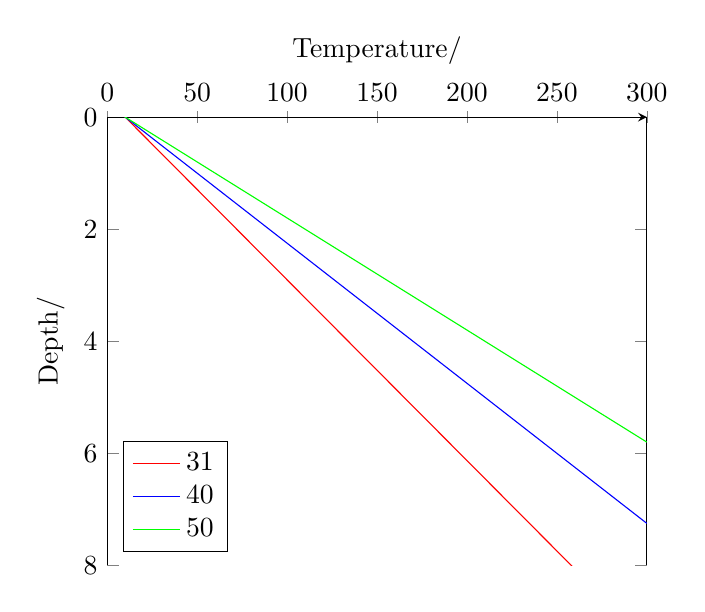
\begin{tikzpicture}
    \begin{axis}[y dir = {reverse},
                 xlabel = {Temperature/\unit{\degreeCelsius}},
                 ylabel = {Depth/\unit{\km}},
                 xmin = 0,
                 xmax = 300,
                 ymin = 0,
                 ymax = 8,
                 axis x line=top,
                 legend style={at={(0.03,0.03)}, anchor=south west},]
        \addplot[color=red,domain=0:300]{(x-10)/31};
        \addlegendentry{\qty{31}{\degreeCelsius\per\km}}
        \addplot[color=blue,domain=0:300]{(x-10)/40};
        \addlegendentry{\qty{40}{\degreeCelsius\per\km}}
        \addplot[color=green,domain=0:300]{(x-10)/50};
        \addlegendentry{\qty{50}{\degreeCelsius\per\km}}
    \end{axis}
\end{tikzpicture}
        \caption{The sub-surface temperature for different geothermal gradients}
        \label{fig:GeothermalGradient}
    \end{figure}

    The geothermal gradient is closely linked to the heat flux in the sub-surface, which in turn is strongly dependent on geological and tectonic setting. For example, in compressional settings, where two plates move towards one another, subduction can lead to a partial melting of the subdued plate and the creation of magmatic zones near the surface, raising the heat flux. Subduction, has led to geothermal resources in most land masses bordering the Pacific, Cocos and Nazca tectonic plates. Similarly, in extensional settings, rifting, where two plates move apart from one another with the gap being filled with material from the astenosphere, and thinning of the plate itself can increase the local heat flux. Rifting has led to geothermal resources in Iceland, the Azores and East Africa, while thinning has given rise to the non-magmatic geothermal Basin and Range region in Nevada, United State, \cite{DiPippo2016}.

    Ultimately, the geothermal gradient is highly site specific and may not be linear. For example, faults may provide preferential fluid pathways, thus allowing hot fluids to reach shallower depths raising the local temperature.  

\section{Geothermal Systems}
\label{sec:geothermal_systems}
    The following section aims to provide background on the three main types of geothermal systems and the make-up of geothermal fluids.

    \subsection{Hydrothermal Systems}
    \label{sec:hydrothermal_system}
    There are many naturally occurring geothermal systems, more commonly referred to as \emph{hydrothermal systems}, see Figure~\ref{fig:HydrothermalSystem}. 
    
    In hydrothermal systems, surface water (e.g. precipitation) percolates into the sub-surface via faults and fractures under the force of gravity (A to B), which provide low-resistance pathway deep into the Earth. At some depth, these pathways may intersect a formation of even lower resistance, causing the fluid to preferentially flow into this formation. In the presence of a heat source, the fluid begins to heat up and rise, due to its reducing density with temperature (B to C). Other high permeability faults intersecting the formation, then provide a low-resistance pathway back to the surface (C to E). The difference in density between the hot fluid and cold fluid, results in a higher potentiometric surface for the hot fluid allowing the fluid to naturally circulate - this is commonly referred to as a \emph{thermosiphon}. At the surface the fluid then enters the Water Cycle and is eventually returned in the form of precipitation, closing the loop (E to A).  
    
    Depending on the temperature of the heat source (F), the fluid may arrive at the surface as a liquid, or, if the fluid  pressure drops to the fluids saturation pressure (D), as a vapour, or vapour-liquid two-phase mixture. The presence of such hydrothermal systems can most commonly be deduced from surface features such as fumaroles, hot springs, mud pits, geysers etc. and are still an important instrument in the discovery of geothermal resources today.

    % schematic of a hydrothermal system
    \begin{figure}[H]
        \centering
        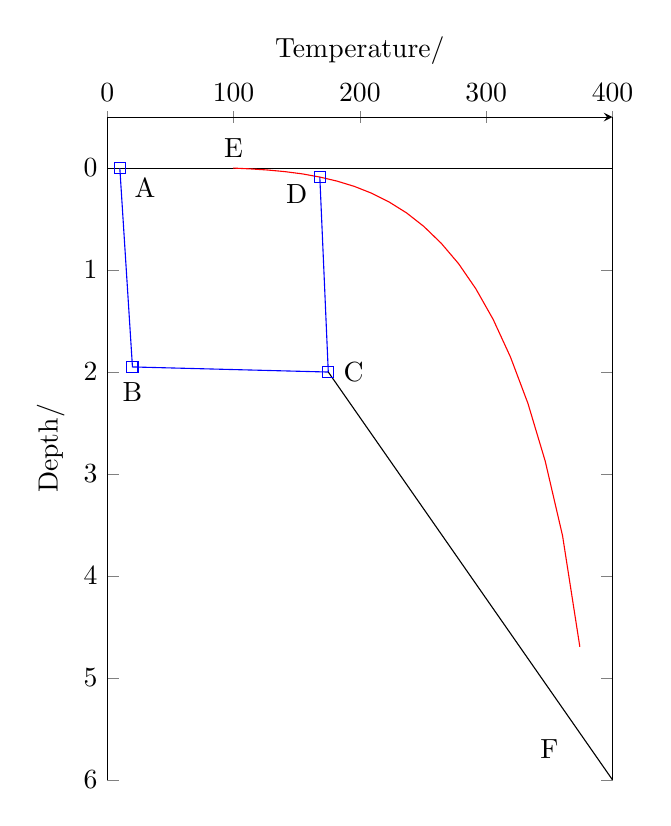
\begin{tikzpicture}[baseline]
    \begin{axis}[y dir = {reverse},
                 xlabel = {Temperature/\unit{\degreeCelsius}},
                 ylabel = {Depth/\unit{\km}},
                 xmin = 0,
                 xmax = 400,
                 ymin = -0.5,
                 ymax = 6,
                 axis x line=top,
                 legend style={at={(0.5,-0.03)}, anchor=north},
                 height=10cm,
                 width=8cm]
        \addplot[color=black]
            coordinates {(0,0)(400,0)};
        
        \addplot[color=red]
            coordinates {(99.6,0.000)  (113.4,0.008)  (127.1,0.019)  (140.8,0.035)  (154.5,0.057)  (168.3,0.088)  (182.0,0.128)  (195.7,0.180)  (209.4,0.247)  (223.2,0.333)  (236.9,0.439)  (250.6,0.572)  (264.3,0.736)  (278.1,0.937)  (291.8,1.184)  (305.5,1.484)  (319.2,1.853)  (333.0,2.307)  (346.7,2.874)  (360.4,3.604)  (374.1,4.694)};
            
        \addplot[color=blue,mark=square]
            coordinates {(10,0)(20,1.95)(175,2)(168.3,0.088)};
        \node at (axis cs:30,0.2) [] {A};
        \node at (axis cs:20,2.2) [] {B};
        \node at (axis cs:195,2) [] {C};
        \node at (axis cs:150,0.25) [] {D};
        \node at (axis cs:100,-0.2) [] {E};
        
        \addplot[color=black]
            coordinates {(400,6)(175,2)};
        \node at (axis cs:350,5.7) [] {F};
            
    \end{axis}
\end{tikzpicture}%
~%
%
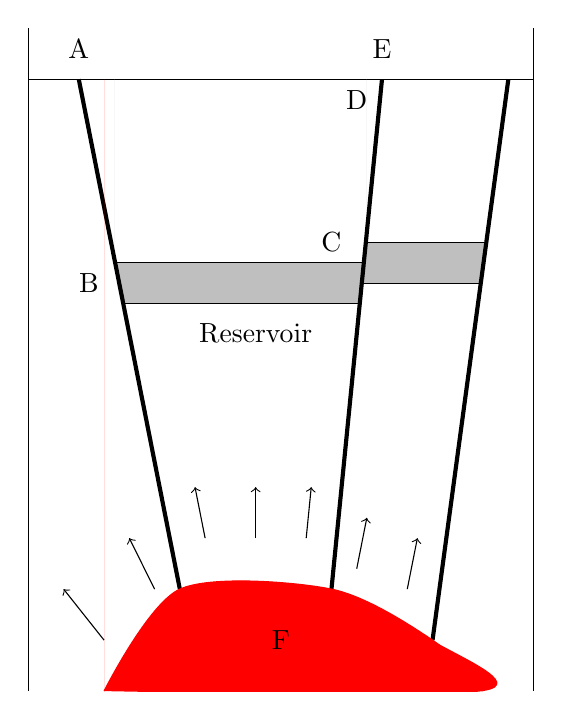
\begin{tikzpicture}[baseline]
    \begin{axis}[y dir = {reverse},
                 xmin = 0,
                 xmax = 100,
                 ymin = -0.5,
                 ymax = 6,
                 axis x line=top,
                 axis x line=none,
                 legend style={at={(0.03,0.03)}, anchor=south west},
                  height=10cm,
                 width=8cm,
                 ticks=none]
        % add the surface
        \addplot[color=black]
            coordinates {(0,0)(400,0)};
            
        % adding the reservoir
        \addplot[fill=lightgray,draw=none] coordinates {(17,1.8) (18.5,2.2) (65.5,2.2) (66.5,1.8) (17, 1.8)} \closedcycle;
        \addplot[color=black]
            coordinates {(17,1.8)(66,1.8)};
        \addplot[color=black]
            coordinates {(19,2.2) (66,2.2)};
        \node at (axis cs:45,2.3) [anchor=north] {Reservoir};

        \addplot[fill=lightgray,draw=none] coordinates {(67,1.6) (66,2.0) (89.5,2.0) (91,1.6) (67, 1.6)} \closedcycle;
        \addplot[color=black]
            coordinates {(67,1.6)(91,1.6)};
        \addplot[color=black]
            coordinates {(66,2.0) (90,2.0)};

        % adding the faults
        \addplot[color=black, line width=1.5pt]
            coordinates {(10,0)(30,5)};
        \addplot[color=black, line width=1.5pt]
            coordinates {(60,5) (70,0)};
        \addplot[color=black, line width=1.5pt]
            coordinates {(80,5.5) (95,0)};

        % adding the heat source
        \addplot[fill=red,draw=none, smooth] coordinates {(15,6) (30,5) (60,5) (80,5.5) (90, 6) (15, 6)} \closedcycle;
        \addplot[smooth,color=red]
            coordinates {(15,6)(30,5)(60,5)(80,5.5)(90,6)};
        \node at (axis cs:50,5.5) [color=black] {F};

        % adding the fluid pathway
        \node at (axis cs:10,-0.3) [] {A};
        \node at (axis cs:12,2) [] {B};
        \node at (axis cs:60,1.6) [] {C};
        \node at (axis cs:65,0.2) [] {D};
        \node at (axis cs:70,-0.3) [] {E};

        % add conduction arrows
        \draw[->](axis cs:15,5.5)--(axis cs:7,5);
        \draw[->](axis cs:25,5)--(axis cs:20,4.5);
        \draw[->](axis cs:35,4.5)--(axis cs:33,4);
        \draw[->](axis cs:45,4.5)--(axis cs:45,4);
        \draw[->](axis cs:55,4.5)--(axis cs:56,4);
        \draw[->](axis cs:65,4.8)--(axis cs:67,4.3);
        \draw[->](axis cs:75,5)--(axis cs:77,4.5);
        
    \end{axis}
\end{tikzpicture}        
        \caption[Schematic of a hydrothermal system]{Schematic of a hydrothermal system. Left, the fluid path and temperature (blue), the saturation curve (red), and the conduction from the heat source (black). Right, the geological cross-section showing the faults (black), the reservoir (grey), the heat source (red) and the condition from the heat source. Graphic adapted from \citeauthor{kruger1973} \cite{kruger1973} and \citeauthor{DiPippo2016} \cite{DiPippo2016}.}
        \label{fig:HydrothermalSystem}
    \end{figure}

    In summary, the key features of a hydrothermal system are the heat source, the reservoir, a supply of water to extract the heat and a recharge mechanism to replenish the produced water.

    In a commercial setting, hydrothermal systems are typically exploited by drilling two wellbores into the reservoir; one to produce the hot fluid to surface, and the other to re-inject the cold fluid into the reservoir - this is commonly called a \emph{doublet}. The wellbores essentially replace the faults as the low-resistance pathways for the fluid to/from the reservoir. 
    
    Where the formation pressure is insufficient for the fluid to reach the surface, pumps may be used to pressurise the fluid and deliver it to the surface. However, pumps need to be installed below the flash-point to avoid cavitation, which can damage the pump internal components. There are two different types of pumps, \acp{ESP} where the motor is located within the wellbore and is cooled by the fluid rushing past it, and \acp{LSP}, where the motor is located at the surface and drives the impeller via a continuous shaft. To prevent overheating of the motor the use of \acp{ESP} is limited to lower temperature applications. On the other hand, the application of \acp{LSP} is limited by the length of the shaft and the requirement for a vertical wellbore.       

    \subsection{Enhanced Geothermal Systems}
    \label{sec:enhanced_geothermal_systems}

    Due to the generally increasing temperature with depth, deeper geothermal systems tend to be more sought after, however, may not display sufficient, if any, permeability to allow circulation of fluids through the formation. \ac{EGS} seek to address this issue by using stimulation techniques, such as hydraulic fracturing or hydro-shearing to create or re-activate fracture networks within the rock to allow the circulation of fluids, and therefore the extraction of heat. Although the idea was first presented in the 1970s, \cite{Potter1974}, and has been shown to be technically feasible, to date there are only few commercially active \ac{EGS} sites, such as Soultz-sous-Forêts\cite{ES2024}, or Rittershoffen \cite{ES2024}. Utah FORGE is a prominent research initiative into EGS \cite{UtahForge2024}.

    The main challenges preventing commercial adoption of EGS are:
    \begin{itemize}
        \item \emph{Induced Seismicity} - the circulation of fluids may reactivate the fracture network, causing low magnitude tremors felt at the surface that may in some cases damage buildings, as was the case at a potential \ac{EGS} site in Basel in 2006 \cite{Deichmann2009}.
        \item \emph{Flow Rates} - the circulation rates must be sufficiently high for the project to reach an economically viable scale, however this reduces the residence time within the formation and may result in incomplete heating of the fluid. 
        \item \emph{Clogging} - over time scales and other particulates can clogging parts of the fracture network reducing the overall permeability and in turn limit the flow rates and heat removal \cite{LuoKottsova2023}.
        \item \emph{Early Thermal Breakthrough} - enhanced geothermal systems are typically smaller than hydrothermal systems and thus at equal heat removal, the EGS will be exhausted sooner.
    \end{itemize}
    
    \subsection{Advanced Geothermal Systems}
    \label{sec:stimulation}

    Unlike Hydrothermal systems or EGS, where the fluid is in direct contact with the formation, in advanced geothermal systems, a self-contained network of wellbores is used to extract the heat from the reservoir, with the fluid being contained within the closed-loop at all times. This configuration has as several advantages over hydrothermal and EGS systems as it reduces the dependence on the formation properties, which pose a major source of uncertainty for any geothermal project. More over, as the working fluid is fully contained within the wellbore at all times, the risk of induced seismicity or contamination of drinking water aquifers is all but eliminated. %and other concerns such as contamination of drinking water aquifers.
    
    While there are some demonstration and test sites (e.g. Geretsriede, Germany), the long-term commercial viability of these systems has not yet been proven. Particularly, due to the significant drilling required for these systems and the lower rate of heat transfer posing a potential limitation on the scale \cite{Malek2022, Beckers2022}.

    \subsection{Geothermal Fluid}
    \label{sec:geothermal_fluid}
        The working fluid in geothermal energy extraction is typically the in-situ reservoir fluid, which is primarily comprised of water, but may also contain dissolved minerals and gases. To avoid confusion with the power plant working fluid, it is often referred to a \emph{geofluid} or \emph{brine}. The geofluid composition is derived from the fluids present when the formation was first deposited, the chemical equilibration with the formation over geological timescales, as well as the migrations of tertiary fluids (e.g. methane) into the formation.

        Changes in temperature and pressure (e.g. by producing the geofluid to surface and extracting its heat) or composition (e.g. injection of water), disturb the geofluid's chemical equilibrium, which can lead to the precipitation of dissolved species. In the case of solid species, this mineralisation, also commonly referred to as \emph{scaling}, poses serious operational issues as the scales can deposit in all parts of the production system and pose an additional resistance to flow and heat transfer. Scaling can be controlled through chemical inhibitors or ensuring that temperatures and pressures make mineralisation thermodynamically unfavourable.

        Dissolved gases also pose an important operational challenge, as they can be harmful and toxic (e.g. Hydrogen Sulphide, \ce{H2S}, or Mercury, \ce{Hg}), have a global warming potential (e.g. carbon dioxide, \ce{CO2}, or methane, \ce{CH4}), or have a strong odour (e.g. Hydrogen Sulphide, \ce{H2S}). Collectively these gases are commonly referred to as \ac{NCG} because they cannot be liquefied at ambient or near-ambient conditions, making their handling costly. Common issues and technological options related to the handling of \ac{NCG} will be dealt with in more detail in Section~\ref{sec:litrev_NCG_handling}.
    
\section{Geothermal Power Generation}
\label{sec:geothermal_power}
    Where geothermal resources are hot enough, it is possible to convert the thermal energy into electrical energy. This is achieved using two different power plant technologies; \ac{DSC} and binary cycle power plants. The below sees to provide an overview of the most prominent types of geothermal power plants.

    \subsection{Direct Steam Cycle: Dry Steam}
    \label{sec:dry_steam}
        Dry steam plants operate on the highest enthalpy resources, where the geofluid arrives at the surface as a  saturated vapour. While they are the earliest examples of geothermal power plant, the specific geological conditions required for fully vapourised geofluids mean that there are only a small number of these sites globally. The most prominent dry steam power plants are those at Lardarello, Italy, or The Geysers, USA, \cite{DiPippo2016}.  
        
        The steam is then expanded in a turbine, which drives a generator to generate electricity. The low-pressure steam from the turbine is then cooled condensed to separate the \ac{NCG}, which is then treated (not pictured) to remove pollutants (e.g. \ce{H2S}) before typically being vented to the atmosphere. The liquid is re-injected into the geothermal reservoir to minimise pressure decline in the reservoir and maximise the lifetime of the resource. Figure~\ref{fig:schematic_dry_steam} provides a schematic of a dry steam geothermal power plant.

        As of 2016, there were a total of \num{68} dry steam geothermal power plants across the United States, Italy, Indonesia, Japan, Iceland and New Zealand, producing a total of \qty{2.87}{\giga\watt}, representing \qty{24.0}{\percent} of total geothermal power production \cite{DiPippo2016}.

        \begin{figure}[H]
            \centering
            \begin{tikzpicture}
    % draw equipment
    \pic (producer) at (0,0) {producer};
    \pic (solids) [scale=0.25] at ($(producer-anchor) + (1.5, 2)$) {block};
    \pic (moist) [scale=0.3, rotate=90] at ($(solids-anchor) + (2, 0)$) {block};
    \pic (turbine) at ($(moist-anchor) + (2, 0)$) {turbine_gen};
    \pic (condenser) at ($(turbine-anchor) + (3, -1.25)$) {condenser};
    \pic[scale=0.4] (NCGsep) at ($(condenser-anchor) + (2.5, +0.5)$) {gas-liquid separator};
    \pic (injector) at ($(NCGsep-anchor) + (0, -1.25)$) {injector};
    \pic (treat) [scale=0.25] at ($(NCGsep-gas outlet) + (1.5, 2)$) {block};

    % draw connectors
    \draw[main stream] (producer-top) |- (solids-left);
    \draw[main stream] (solids-right) -- (moist-top);
    \draw[main stream] (solids-bottom) -- ++ (0,-0.5);
    \draw[main stream] (moist-right) -| (turbine-inlet top);
    \draw[main stream] (moist-left) -- ++ (0, -0.5);
    \draw[main stream] (turbine-outlet bottom) |- (condenser-pipes inlet);
    \draw[main stream] (condenser-pipes outlet) -- (NCGsep-inlet left);
    \draw[main stream] (NCGsep-liquid outlet) -- (injector-top);
    \draw[main stream] (NCGsep-gas outlet) |- (treat-left);
    \draw[main stream] (treat-right) -- ++ (1.5,0);

    % draw labels
    \node[below] at (producer-bottom) {Producer};
    \node[above, align=center] at (solids-top) {Solids\\Removal};
    \node[above, align=center] at (moist-right) {Moisture\\Removal};
    \node[above] at (turbine-top) {Turbine};
    \node[right] at (turbine-right) {Generator};
    \node[below] at (condenser-bottom) {Condenser};
    \node[right] at (NCGsep-inlet right) {NCG separator};
    \node[below] at (injector-bottom) {Injector};
    \node[below, align=center] at (treat-bottom) {NCG\\Treatment};
    \node[above] at ($(treat-top) + ((1.5, 0)$) {To atmosphere};

\end{tikzpicture}
            \caption[Schematic of a dry steam geothermal power plant.]{Schematic of a dry steam geothermal power plant. Adapted from \cite{DiPippo2016}}
            \label{fig:schematic_dry_steam}
        \end{figure}
    
    \subsection{Direct Steam Cycle: Flash}
    \label{sec:flash}

        Flash plants operate on lower enthalpy resources, where the geofluid arrives at the surface either as a liquid or low vapour quality. As such, the geological requirements for flash power plants are far less niche compared to dry steam plants.

        The hot geofluid, single phase liquid or a vapour-liquid mixture, is expanded in a valve to liberate more vapour, which is then separated from the liquid and sent to the turbine. In the turbine the vapour is expanded further, which drives a generator and generates electricity. The low-pressure steam is then condensed and the \ac{NCG} is removed from the condenser and then treated (not pictured) to remove pollutants (e.g. \ce{H2S}) before typically being vented to the atmosphere. The condensate is repressurised and then, together with the left-over brine, re-injected into the reservoir. Figure~\ref{fig:schematic_dry_steam} provides a schematic of a flash geothermal power plant.
    
        \begin{figure}[H]
            \centering
            \begin{tikzpicture}
    % draw equipment
    \pic (producer) at (0,0) {producer};
    \pic (valve) at ($(producer-anchor) + (1.5, 2.5)$) {lamination valve};
    \pic[scale=0.4] (separator) at ($(valve-anchor) + (2, 0)$) {gas-liquid separator};
    \pic (turbine) at ($(separator-anchor) + (3, 1.5)$) {turbine_gen};
    \pic (condenser) at ($(turbine-anchor) + (2, -1.5)$) {condenser};
    \pic[scale=0.4] (NCGsep) at ($(condenser-anchor) + (3, 0.5)$) {gas-liquid separator};
    \pic (condpump) at ($(condenser-anchor) + (0, -2.3)$) {centrifugal pump};
    \pic (injector) at ($0.5*(producer-anchor) + 0.5*(condpump-anchor)$) {injector};
    \pic[rotate=180] (joint) at ($(injector-anchor) + (0, 1)$) {valve triple=main};
    
    
    % % draw connectors
    \draw[main stream] (producer-top) |- (valve-inlet);
    \draw[main stream] (valve-outlet) -- (separator-inlet left);
    \draw[main stream] (separator-gas outlet) |- (turbine-inlet top);
    \draw[main stream] (turbine-outlet bottom) |- (condenser-pipes inlet);
    \draw[main stream] (condenser-pipes outlet) -- (NCGsep-inlet left);
    \draw[main stream] (NCGsep-gas outlet) |- ++ (1,1);
    \draw[main stream] (NCGsep-liquid outlet) |- (condpump-anchor);
    
    \draw[main stream] (condpump-top) |- (joint-left);
    \draw[main stream] (separator-liquid outlet) |- (joint-right);
    \draw[main stream] (joint-top) -- (injector-top);

    % % draw labels
    \node[below] at (producer-bottom) {Producer};
    \node[above, align=center] at (valve-top) {Expansion\\ Valve};
    \node[right, align=left] at (separator-inlet right) {Steam \\ Separator};
    \node[above] at (turbine-top) {Turbine};
    \node[right] at (turbine-right) {Generator};
    \node[below] at (condenser-bottom) {Condenser};
    \node[right, align=left] at (NCGsep-inlet right) {NCG \\ separator};
    \node[above right] at ($(NCGsep-gas outlet) + ((0, 1)$) {To atmosphere};
    \node[below] at (condpump-bottom) {Condensate Pump};
    \node[below] at (injector-bottom) {Injector};

\end{tikzpicture}
            \caption[Schematic of a direct steam cycle with flash geothermal power plant.]{Schematic of a direct steam cycle with flash geothermal power plant. Adapted from \cite{DiPippo2016}}
            \label{fig:schematic_flash}
        \end{figure}

        The degree of flashing is a compromise between liberating more steam from the geofluid and specific enthalpy change across the turbine. Additional flashing stages can be used to liberate more vapour from the geofluid, see Figure~\ref{fig:schematic_dual_flash}. While such \emph{dual-flash} plants are quite common, there only exist a handful of \emph{triple-flash} plants \cite{DiPippo2016}.

        \begin{figure}[H]
            \centering
            \begin{tikzpicture}
    % draw equipment
    \pic (producer) at (0,0) {producer};
    
    \pic (valve) at ($(producer-anchor) + (1.5, 3.5)$) {lamination valve};
    \pic[scale=0.4] (separator) at ($(valve-anchor) + (2, 0)$) {gas-liquid separator};
    \pic (valve_lp) at ($(separator-liquid outlet) + (1.5, -0.5)$) {lamination valve};
    \pic[scale=0.4] (separator_lp) at ($(valve_lp-anchor) + (1.5, 0)$) {gas-liquid separator};

    \pic (turbine) at ($(separator-anchor) + (2.6, 2)$) {multi_turbine_gen};
    \pic (condenser) at ($(turbine-anchor) + (3, -1.2)$) {condenser};
    \pic[scale=0.4] (NCGsep) at ($(condenser-anchor) + (2, 0.5)$) {gas-liquid separator};
    
    \pic (injector) at ($(producer-anchor) + (6.5,0)$) {injector};
    \pic (condpump) at ($(injector-anchor) + (3, 0.2)$) {centrifugal pump};
    \pic[rotate=270] (joint) at ($(injector-anchor) + (0, 1)$) {valve triple=main};
    
    
    % % draw connectors
    \draw[main stream] (producer-top) |- (valve-inlet);
    \draw[main stream] (valve-outlet) -- (separator-inlet left);
    \draw[main stream] (separator-gas outlet) |- (turbine-inlet_hp top);
    
    \draw[main stream] (separator-liquid outlet) |- (valve_lp-inlet);
    \draw[main stream] (valve_lp-inlet) -- (separator_lp-inlet left);
    \draw[main stream] (separator_lp-gas outlet) -- (turbine-inlet_lp bottom);

    \draw[main stream] (turbine-outlet_lp bottom) |- (condenser-pipes inlet);

    \draw[main stream] (condenser-pipes outlet) -- (NCGsep-inlet left);
    \draw[main stream] (NCGsep-gas outlet) |- ++ (1,1);
    \draw[main stream] (NCGsep-liquid outlet) |- (condpump-anchor);
    
    \draw[main stream] (condpump-top) |- (joint-top);
    \draw[main stream] (separator_lp-liquid outlet) -- (joint-left);
    \draw[main stream] (joint-right) -- (injector-top);

    % % draw labels
    \node[below] at (producer-bottom) {Producer};
    \node[above, align=center] at (valve-top) {Expansion\\ Valve};
    \node[right, align=left] at (separator-inlet right) {HP Steam \\ Separator};
    \node[right, align=left] at (separator_lp-inlet right) {LP Steam \\ Separator};
    \node[above] at (turbine-top) {Turbine};
    \node[right] at (turbine-right) {Generator};
    \node[below] at (condenser-bottom) {Condenser};
    \node[right, align=left] at (NCGsep-inlet right) {NCG \\ separator};
    \node[above right] at ($(NCGsep-gas outlet) + ((0, 1)$) {To atmosphere};
    \node[below] at (condpump-bottom) {Condensate Pump};
    \node[below] at (injector-bottom) {Injector};

\end{tikzpicture}
            \caption[Schematic of a direct steam cycle with double flash geothermal power plant.]{Schematic of a direct steam cycle with double flash geothermal power plant. Adapted from \cite{DiPippo2016}}
            \label{fig:schematic_dual_flash}
        \end{figure}

        As of 2016, there were a total of \num{243} flash geothermal power plants across the Philipines, the United States, Mexico, Indonisia, Iceland, Japan and Kenya, producing a total of \qty{7.33}{\giga\watt}, representing \qty{61.4}{\percent} of total geothermal power production \cite{DiPippo2016}.

    \subsection{Binary Cycle}
    \label{sec:binary_cycle}

        Binary plants allow the exploitation of low-enthalpy geothermal resources, no or insuffucient vapour can be generated for commercial operation of a flash plant - this has opened a great number of otherwise uneconomical resources up for exploitation.

        In a binary power plant, see Figure~\ref{fig:schematic_binary} the hot geofluid is used to heat and evaporate a secondary fluid, also referred to as the cycle working fluid, or colloquially \emph{working fluid}. The working fluid vapour is then expanded in a turbine, which drives a generator to generate electricity. The low pressure vapour is then condensed, re-pressurised and then returned to the pre-heater inlet, closing the loop. A recuperator may be used to recover heat from the working fluid leaving the turbine, and to use it to partially pre-heating the working fluid.

        \begin{figure}[H]
            \centering
            \begin{tikzpicture}
    % draw equipment
    \pic (producer) at (0,0) {producer};
    \pic (injector) at (2,0) {injector};
    
    \pic[rotate=180] (preheater) at ($(injector-anchor) + (0.925, 2)$) {heat exchanger biphase};
    \pic[rotate=180] (evaporator) at ($(preheater-anchor) + (0, 1.5)$) {heat exchanger biphase};
    \pic[rotate=180] (superheater) at ($(evaporator-anchor) + (0, 1.5)$) {heat exchanger biphase};
    
    \pic (turbine) at ($(superheater-anchor) + (4, 0.5)$) {turbine_gen};
    \pic[rotate=180] (recuperator) at ($(turbine-outlet bottom) + (0, -3.8)$) {heat exchanger};
    \pic (condenser) at ($(recuperator-anchor) + (2, -1)$) {condenser};
    \pic (pump) at ($(condenser-anchor) + (2.5, 0.5)$) {centrifugal pump};
    
    % % draw connectors
    \draw[main stream] (producer-top) |- (superheater-pipes bottom);
    \draw[main stream] (superheater-pipes top) 
        -- ($(superheater-pipes top) + (-0.5, 0)$) 
        |- (evaporator-pipes bottom);
    \draw[main stream] (evaporator-pipes top) 
        -- ($(evaporator-pipes top) + (-0.5, 0)$) 
        |- (preheater-pipes bottom);
    \draw[main stream] (preheater-pipes top) 
        -| ($(preheater-pipes top) + (-0.5, -1)$) 
        -- (injector-top);

    \draw[main stream] (preheater-shell bottom) -- (evaporator-shell top);
    \draw[main stream] (evaporator-shell bottom) -- (superheater-shell top);
    \draw[main stream] (superheater-shell bottom) |- (turbine-inlet top);

    \draw[main stream] (turbine-outlet bottom) -- (recuperator-shell bottom);
    \draw[main stream] (recuperator-shell top) |- (condenser-pipes inlet);
    \draw[main stream] (condenser-pipes outlet) -- (pump-anchor);
    \draw[main stream] (pump-top) |- (recuperator-pipes left);
    \draw[main stream] (recuperator-pipes right) -| (preheater-shell top);
    
    % % draw labels
    \node[below] at (producer-bottom) {Producer};
    \node[right] at (preheater-shell left) {Pre-Heater};
    \node[right] at (evaporator-shell left) {Evaporator};
    \node[right] at (superheater-shell left) {Super-Heater};
    \node[above] at (turbine-top) {Turbine};
    \node[right] at (turbine-right) {Generator};
    \node[below, align=left] at (condenser-bottom) {Condenser};
    \node[below, align=center] at (pump-bottom) {Circulation \\ Pump};
    \node[below] at (injector-bottom) {Injector};
    \node[above right] at (recuperator-pipes left) {Recuperator (opt.)};


\end{tikzpicture}
            \caption[Schematic of a binary ORC geothermal power plant.]{Schematic of a binary ORC geothermal power plant. Adapted from \cite{DiPippo2016}}
            \label{fig:schematic_binary}
        \end{figure}

        The most popular type of binary geothermal plant use an \ac{ORC}, where the working fluid is some organic fluid, typically a hydrocarbon or a refrigerant. Another example of a binary cycle, is the Kalina cycle, which uses a mixture of water and ammonia mixture as the working fluid, however there are currently only a small number of active power plants using this cycle configuration (e.g. Húsavík in Iceland \cite{Husavik2024} or Bruchsal in Germany \cite{EnBW2024}).

        As of 2016, there were a total of \num{203} binary geothermal power plants across the United States, New Zealand, Turkey, Kenya, Guatemala and the Philipines, producing a total of \qty{1.25}{\giga\watt}, representing \qty{10.4}{\percent} of total geothermal power production \cite{DiPippo2016}. 
        
    % \subsection{Challenges for Geothermal Power Generation}
    %     \label{sec:challenges}
        
    
    %     \begin{itemize}
    %         \item low efficiency
    %         \item handling of corrosive geofluids
    %         \item handling of NCG
    %         \item thermophysical properties of geofluids
    %         \item public acceptance
    %     \end{itemize}
    
\section{Research Objectives}
\label{sec:research_objectives}
    The global objective of this work is to investigate electrical power generation from two-phase geothermal heat sources using both binary \ac{ORC} and \ac{DSC} technology in an effort to establish thermodynamic and techno-economic application envelopes. Here, the effect of impurities, such as \ac{NCG}, on power generation, as well as the parasitic losses associated with the disposal of \ac{NCG} is an area of interest, and could represent a novel-niche for binary \ac{ORC} geothermal power. To assess the thermodynamic and techno-economic performance of these two technologies, a holistic model of the geofluid, power plant and economics is required. 

    Thus, the three key research objectives are the:
    \begin{enumerate}
        \item Curation or development of a reliable and robust methodology for modelling the thermophysical properties and phase behaviour of real geofluids (i.e. water and \ac{NCG}, water and salts, water and salts and \ac{NCG}.
        \item Curation or development of a simulation tool to evaluate the thermodynamic and techno-economic performance of both \ac{DSC} and binary \ac{ORC} geothermal power plants.
        \item Evaluation and comparison of the thermodynamic and techno-economic performance of \ac{DSC} and binary \ac{ORC} geothermal power plants for ideal and real geofluids (i.e. pure water and water with \ac{NCG} respectively), including different disposal scenarios for co-produced \ac{NCG}. 
    \end{enumerate}
    
\section{Project Outline}
\label{sec:project_outline}

    Chapter \ref{ch:thermophysmodelling} covers the review of existing thermophysical property modelling approaches and the development of \emph{GeoProp}

    Chapter \ref{ch:power_generation} provides technical background on key aspects of geothermal power generation, including the different power plant technologies, turbines, heat exchangers, as well as equipment costs.

    Chapter \ref{ch:PowerCycle} documents the development of \emph{PowerCycle}, detailing the component performance and cost models as well as their validation.

    The investigations into the thermodynamic and techno-economic performance of binary \ac{ORC} and single flash \ac{DSC} geothermal power plants, as well as the impact of impurities and their handling are covered in chapter \ref{ch:process_simulation}.

    Conclusions are summarised in chapter \ref{ch:conclusions}.

    Appendix \ref{ch:appendix_a} provides supplementary information on the thermodynamic criteria for chemical equilibrium. Appendix \ref{ch:appendix_b} details the implementation of the \ac{SP2009} partitioning model and changes to the original model. Appendix \ref{ch:appendix_c} details the governing equation for the second law performance analysis. Appendix \ref{ch:appendix_d} provides code examples for the use of \emph{GeoProp}, and finally, appendix \ref{ch:appendix_f} provides additional validations for \emph{PowerCycle} component models.
    